% file: 01-pattern-even.tex

\documentclass[tikz]{standalone}
\usetikzlibrary{decorations.pathreplacing, positioning, arrows.meta, shapes.multipart, calc}

\begin{document}
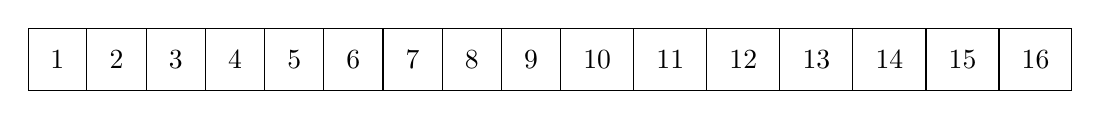
\begin{tikzpicture}[Array/.style = {rectangle split, rectangle split parts = #1, rectangle split horizontal,
    inner sep = 8pt, anchor = center}]
    % bit array
    % \node[Array = {16}, draw] (A) 
    %   {\nodepart{two}\nodepart{three}\nodepart{four}\nodepart{five}\nodepart{six}\nodepart{seven}\nodepart{eight}\nodepart{nine}
    %    \nodepart{ten}\nodepart{eleven}\nodepart{twelve}\nodepart{thirteen}\nodepart{fourteen}\nodepart{fifteen}\nodepart{sixteen}};

    % index
    \node[Array = {16}, draw] (A-index) 
      {1\nodepart{two}2\nodepart{three}3\nodepart{four}4\nodepart{five}5\nodepart{six}6\nodepart{seven}7\nodepart{eight}8\nodepart{nine}9
       \nodepart{ten}10\nodepart{eleven}11\nodepart{twelve}12\nodepart{thirteen}13\nodepart{fourteen}14\nodepart{fifteen}15\nodepart{sixteen}16};
\end{tikzpicture}
\end{document}
